\documentclass[12pt,a4paper]{article}

\usepackage{amsmath,amssymb,amsthm}
\usepackage{mathtools}
\usepackage{geometry}
\usepackage{hyperref}
\usepackage[protrusion=true,expansion=false]{microtype}
\usepackage{setspace}
\usepackage{enumitem}
\usepackage{tikz}
\usepackage{tikz-cd}
\usetikzlibrary{positioning,arrows,arrows.meta,calc,matrix}
\usepackage{booktabs}
\usepackage{array}
\usepackage{caption}
\usepackage{subcaption}
\usepackage{xcolor}
\usepackage[T1]{fontenc}
\usepackage[utf8]{inputenc}

\geometry{
  top=1.1in,
  bottom=1.1in,
  left=1.25in,
  right=1.25in
}

\onehalfspacing

\hypersetup{
  colorlinks=true,
  linkcolor=black,
  citecolor=black,
  urlcolor=black
}

\theoremstyle{plain}
\newtheorem{theorem}{Theorem}[section]
\newtheorem{proposition}[theorem]{Proposition}
\newtheorem{lemma}[theorem]{Lemma}
\newtheorem{corollary}[theorem]{Corollary}

\theoremstyle{definition}
\newtheorem{definition}[theorem]{Definition}
\newtheorem{example}[theorem]{Example}
\newtheorem{remark}[theorem]{Remark}

\newcommand{\E}{\mathcal{E}}
\newcommand{\B}{\mathcal{B}}
\newcommand{\C}{\mathcal{C}}
\newcommand{\D}{\mathcal{D}}
\newcommand{\Hom}{\mathrm{Hom}}
\newcommand{\id}{\mathrm{id}}
\newcommand{\op}{\mathrm{op}}
\newcommand{\Type}{\mathrm{Type}}
\newcommand{\sign}{\mathrm{sign}}

\title{\textbf{The Geometry of Constraints}\\[0.6em]
\large Adversarial Representations, Fibrational Semantics,\\
and the Dependency Architecture of Formal Systems}

\author{Flyxion}

\date{}

\begin{document}

\maketitle
\thispagestyle{empty}

\begin{abstract}
This essay traces a structural continuity running from the empirical
phenomenon of adversarial vulnerability in machine learning through the
differential geometry of neural representation spaces, and ultimately to
the categorical foundations of dependent type theory. Beginning with the
observation that adversarial perturbations are not isolated anomalies but
geometric features of learned representation manifolds, the essay develops
a unified conceptual framework in which adversarial subspaces, Grothendieck
fibrations, comprehension categories, and the $\lambda$-cube all emerge as
manifestations of the same underlying architecture: a geometry of constraints
governing how structures vary across contexts and interact across levels of
abstraction. The Cox--Bunzel representational similarity framework and
Centered Kernel Alignment are interpreted geometrically as instruments for
probing the foliation structure of high-dimensional semantic manifolds. The
$\lambda$-cube is reinterpreted not as a syntactic taxonomy but as the minimal
coordinate system for a stratified dependency lattice, whose axes correspond to
adjunctions between levels of a formal hierarchy. Comprehension categories are
shown to generate the cube's structure automatically from the minimal data of a
fibration equipped with context extension. Transformer attention mechanisms are
analysed as dynamic metric tensors inducing context-dependent curvature on the
representation manifold. Representation learning is interpreted as a
renormalization flow whose fixed points are the semantic foliations whose
transverse directions constitute the adversarial attack surface. A Geometric
Summary Theorem unifies all of these observations into a single formal
statement. The essay concludes that type theory, categorical semantics,
information geometry, and adversarial machine learning are all partial
descriptions of a single geometry: the geometry of constraint fields defined
over spaces of contexts.
\end{abstract}

\newpage
\tableofcontents
\newpage

%% ======================================================================
\section{Robustness, Regulation, and the Limits of Verification}
%% ======================================================================

Modern neural networks achieve predictive performance that would have appeared
extraordinary a generation ago, yet they remain fragile in a manner that has no
analogue in classical engineering systems. Minor manipulations of input
data---manipulations that appear insignificant or even imperceptible to human
observers---can produce large, discontinuous changes in model behavior. These
adversarial perturbations are not isolated pathological cases. They occupy
large, geometrically structured regions of the input space, and their existence
is not contingent on implementation details of any particular architecture.
They are, as the subsequent analysis will argue, necessary consequences of the
geometry of learned representations in high-dimensional spaces.

This fragility has become a matter not merely of theoretical interest but of
regulatory consequence. As artificial intelligence systems become embedded in
critical infrastructure, financial decision-making, healthcare, and public
governance, their resistance to adversarial manipulation becomes a precondition
of responsible deployment. The European Union's AI Act requires organizations to
demonstrate robustness and security as core properties of high-risk systems.
Similar frameworks are emerging across multiple jurisdictions. Yet these
regulatory demands run immediately into a mathematical obstacle: the adversarial
attack surface of a deep neural network is combinatorially enormous, and
complete verification of robustness with respect to that surface is
computationally infeasible. Even verifying robustness within a small
perturbation radius around a single input is NP-hard in the general case.

The central tension of adversarial machine learning research is therefore not
primarily a tension between safe and unsafe systems but a tension between the
theoretical completeness required by rigorous guarantees and the statistical
coverage achievable in practice. Organizations cannot enumerate all adversarial
inputs. They can only probe the adversarial landscape using surrogate methods
and hope that their probes provide representative coverage. Understanding what
``representative'' means in this context requires understanding the geometry of
representation spaces, which in turn opens onto mathematical structures far
deeper than the applied setting might initially suggest.

This essay traces that depth. It begins with the applied problem of adversarial
transferability and the representational similarity metrics developed to address
it, then passes through the differential geometry of transformer attention
mechanisms and high-dimensional embedding spaces, and ultimately arrives at
Grothendieck fibrations, comprehension categories, and the $\lambda$-cube. The
claim developed throughout is that these apparently disparate topics are unified
by a single structural insight: complex systems, from neural networks to logical
languages, can be understood as layered spaces of states, constraints, and
meta-constraints, and the behavior of adversarial perturbations, program
evaluation, and logical proof are all instances of motion through such layered
spaces.

%% ======================================================================
\section{Geometric Thesis and Essay Roadmap}
%% ======================================================================

The argument of this essay turns on the recognition that three apparently
independent technical domains---adversarial machine learning, dependent type
theory, and categorical semantics---share a common geometric skeleton. Stating
that identification explicitly at the outset will allow the subsequent sections
to be read as coordinate charts on a single underlying structure rather than as
a sequence of loosely related technical expositions.

The three structural parallels are as follows.

The first concerns the degeneracy structure of neural embedding manifolds. A
trained network defines a representation map $h : X \to \mathbb{R}^d$ whose
Jacobian field determines two complementary distributions on the input tangent
bundle: the tangent directions along which representation varies negligibly
(the leaves of the semantic equivalence foliation) and the transverse directions
along which small displacements produce large output changes (the adversarial
subspace). Adversarial vulnerability is the existence of an abundant, wide
adversarial cone in the transverse distribution; robustness corresponds to
minimizing its width or geodesic accessibility from typical data.

The second concerns the fibrational structure of dependent type theory. A
dependent type judgment $\Gamma \vdash A : *$ describes an object in the fiber
of a Grothendieck fibration $p : \E \to \B$ over the context $\Gamma$. A term
inhabiting a dependent type is a section of the resulting bundle. Substitution
is reindexing along base morphisms. Dependent products are right adjoints to
reindexing; dependent sums are left adjoints. Computation is flow along
constraint manifolds; the subject-reduction theorem is the condition that this
flow respects the fibration structure.

The third concerns the categorical structure of comprehension categories and the
$\lambda$-cube. A comprehension category formalizes the minimal data required
for a language to describe objects together with predicates on those objects.
From this minimal data the three axes of the $\lambda$-cube emerge automatically
as the three ways in which the comprehension fibration's levels may depend on
one another. The cube is therefore not a syntactic classification but the
dependency skeleton of any self-describing formal system.

The central thesis of the essay can now be stated precisely.

\begin{quote}
\textit{The degeneracy geometry of neural representation manifolds, the
fibrational semantics of dependent type theory, and the categorical structure
of comprehension categories are all manifestations of the same underlying
phenomenon: constraint fields defined over spaces of contexts, whose sections
describe coherent global objects, whose transverse directions describe
instability, and whose leaf structure encodes the equivalences that the system
has learned or been designed to respect.}
\end{quote}

The essay proceeds as follows. Sections~\ref{sec:transfer}--\ref{sec:foliation}
develop the geometry of adversarial machine learning, from transferability and
CKA through representation manifolds, Jacobian metric structure, and singular
foliations. Section~\ref{sec:attention} analyses transformer attention as a
dynamic metric tensor. Section~\ref{sec:bundles} interprets representation maps
as fiber bundle sections and then as sections of Grothendieck fibrations.
Sections~\ref{sec:cube}--\ref{sec:adjunctions} develop the type-theoretic
material: the $\lambda$-cube as a dependency coordinate system,
comprehension categories, Grothendieck fibrations, and the adjoint lattice
underlying the cube. Sections~\ref{sec:infogeo}--\ref{sec:hott} connect these
structures to information geometry and homotopy type theory.
Section~\ref{sec:renorm} interprets representation learning as a renormalization
flow. Section~\ref{sec:cones} derives adversarial attacks as geodesic escape
from foliation leaves. Section~\ref{sec:summary} states the Geometric Summary
Theorem. Section~\ref{sec:convergence} is the conclusion. The appendix provides
the explicit categorical construction.

%% ======================================================================
\section{Adversarial Transferability and Representational Similarity}
\label{sec:transfer}
%% ======================================================================

The phenomenon of adversarial transferability was among the first indications
that adversarial vulnerability is a structural property of learned
representations rather than an idiosyncratic flaw of individual architectures.
Early work by Goodfellow, Shlens, and Szegedy established that neural networks
exhibit large connected regions of input space in which small perturbations
produce dramatic changes in output classification. These adversarial examples
arise because the learned decision boundary of a network is highly nonlinear
yet locally almost linear in high-dimensional regions. A perturbation aligned
with the gradient of the loss function can push an input across the boundary
with minimal displacement in input space. The fast gradient sign method
formalizes this intuition: given a model $M$ with loss $L_M$ evaluated at
input $x$, the perturbation
\[
\delta_M \;=\; \epsilon\,\sign\!\bigl(\nabla_x L_M(x)\bigr)
\]
produces an adversarial example $x + \delta_M$ that is geometrically close to
$x$ yet behaviorally distant.

The transferability observation sharpened this understanding considerably.
Adversarial examples crafted on one model frequently deceive other models
trained on the same task, even when the architectures differ substantially.
This cross-model transfer implies that adversarial directions are not
idiosyncratic to individual networks but are aligned with structural features
of the shared task geometry. An attack transfers from surrogate $S$ to target
$T$ when the gradients are sufficiently aligned:
\[
\bigl\langle \nabla_x L_S(x),\; \nabla_x L_T(x) \bigr\rangle \;>\; 0.
\]
The question of when this alignment holds, and how to measure it without direct
access to the target model, is the practical problem that representational
similarity metrics are designed to address.

Centered Kernel Alignment (CKA) offers one principled answer. Given two
networks $f$ and $g$ that map a common set of inputs to activation matrices
$X$ and $Y$, CKA measures the similarity between the pairwise relationship
structures induced by these activations. Formally, with $K = XX^\top$ and
$L = YY^\top$,
\[
\mathrm{CKA}(K, L) \;=\; \frac{\|L^\top K\|_F^2}{\|K^\top K\|_F \,\|L^\top L\|_F},
\]
where centering is applied to remove mean effects. CKA produces a value in
$[0,1]$ that is invariant to orthogonal transformations and isotropic scaling.
High CKA similarity indicates that two networks organize data into similar
geometric patterns within their representation spaces. Because adversarial
vulnerabilities are closely tied to the geometry of learned representations,
models with similar CKA scores are more likely to share adversarial directions.

The Cox--Bunzel framework operationalizes this observation into a testing
protocol for organizations required to demonstrate adversarial robustness.
The protocol partitions surrogate models into two groups based on their CKA
similarity to the target model. The high-similarity group, characterized by
CKA scores above approximately $0.55$ for convolutional architectures, provides
proxy models that are geometrically close to the target; attacks generated on
these surrogates are likely to transfer. The low-similarity group, with CKA
scores below approximately $0.35$, ensures that the testing protocol also
explores adversarial regions orthogonal to those shared with the
high-similarity cluster. By combining attacks from both groups, the protocol
approximates coverage of the adversarial landscape without attempting an
impossible exhaustive search. The Diagonal Box Similarity metric supplements
this global picture with layer-by-layer granularity, allowing comparison of
local representation structure at different network depths.

This framework converts the theoretical impossibility of complete robustness
verification into a tractable statistical testing problem. But to understand
why this conversion works---why representational similarity should predict
attack transferability---requires understanding the geometry of the
representation spaces themselves.

%% ======================================================================
\section{The Geometry of Representation Spaces}
%% ======================================================================

Neural networks of sufficient capacity learn to map inputs into
high-dimensional embedding spaces in which semantic relationships become
approximately linear. This approximate linearity is not incidental. It follows
from the interaction between the loss landscape, the implicit biases of gradient
descent, and the functional form of the network.

The resulting representation spaces are not smooth Riemannian manifolds in any
classical sense. A neural network computes a piecewise smooth map from input
space to representation space, assembled from compositions of affine maps and
nonlinearities. The geometry of this map determines the network's sensitivity
to perturbations. At a point $x$ in input space, the Jacobian
\[
J_M(x) \;=\; \frac{\partial h_M(x)}{\partial x}
\]
describes how small displacements in input space propagate into representation
space. When $J_M(x)$ has large singular values along certain directions, small
movements in those directions produce large changes in the representation, and
consequently in the model's output. These high-gain directions constitute the
adversarial subspace local to $x$.

The softmax aggregation inherent in transformer attention also produces a
distinctive geometric phenomenon: many distinct inputs can collapse onto nearly
identical internal representations. The representation space therefore contains
broad regions of approximate equivalence---submanifolds along which the
network's internal state remains nearly constant despite large variation in the
input.

These regions of approximate equivalence form structures resembling degenerate
foliations. A foliation of a manifold is a decomposition into layered
submanifolds of lower dimension, called leaves, that fit together without
crossing. In a standard foliation the leaves are smooth and uniform; in the
degenerate foliations that appear in neural representation spaces, the
dimensionality and smoothness of the leaves vary across the space. Along
directions tangent to the leaves, model behavior remains approximately
invariant. Along directions transverse to the leaves---directions crossing
from one leaf to another---small displacements produce large changes in model
output. The adversarial perturbation problem is precisely the problem of
finding these transverse directions efficiently.

%% ======================================================================
\section{The Metric Structure of Representation Maps}
%% ======================================================================

The foliation interpretation of adversarial subspaces can be made precise by
examining the differential structure induced by the representation map.

Let $h : X \to \mathbb{R}^d$ be the representation map of a trained model,
where $X$ denotes the input space and $\mathbb{R}^d$ the embedding space. The
Jacobian
\[
J_h(x) \;=\; \frac{\partial h(x)}{\partial x}
\]
defines a linear map between tangent spaces
\[
J_h(x) : T_x X \;\longrightarrow\; T_{h(x)} \mathbb{R}^d.
\]
This map induces a pullback metric on the input manifold. If $\langle
\cdot, \cdot \rangle$ denotes the standard inner product in $\mathbb{R}^d$,
the induced metric on $T_x X$ is
\[
g_x(u, v) \;=\; \bigl\langle J_h(x)\,u,\; J_h(x)\,v \bigr\rangle.
\]
The geometry relevant for adversarial perturbations is therefore not the
Euclidean geometry of input space but the Riemannian geometry defined by this
pullback metric. Directions in which the Jacobian has small singular values
correspond to directions along which the representation changes minimally; these
form approximate tangent spaces to the semantic equivalence leaves. Conversely,
directions associated with large singular values correspond to directions in
which representation varies rapidly---precisely the directions in which small
perturbations produce large changes in network output.

The adversarial structure of the model therefore emerges directly from the
spectral geometry of the Jacobian field over the input manifold. Training
implicitly factors the representation space into equivalence classes of inputs
sharing semantic invariants. Two inputs $x$ and $x'$ lie on the same leaf
whenever their downstream classifications agree: $f(h(x)) = f(h(x'))$. The
tangent space to the leaf at $x$ is
\[
T_x \mathcal{F} \;=\; \ker D(f \circ h)_x,
\]
and it is precisely the directions discarded by the Jacobian's low singular
values. The adversarial subspace is the orthogonal complement of this kernel
under $g_x$.

%% ======================================================================
\section{Transformer Attention as a Dynamic Metric Tensor}
\label{sec:attention}
%% ======================================================================

Transformer architectures introduce an additional layer of geometric
complexity through the attention mechanism. Unlike feedforward networks,
where the pullback metric is fixed by the model's parameters, transformer
attention induces a context-dependent metric that varies dynamically with
each input.

For a sequence of token embeddings $H = (h_1, h_2, \dots, h_n)$, the
attention mechanism computes query, key, and value projections
\[
Q = H W_Q, \qquad K = H W_K, \qquad V = H W_V,
\]
and produces the transformed representation
\[
\mathrm{Attn}(H) \;=\;
\mathrm{softmax}\!\left(\frac{Q K^\top}{\sqrt{d_k}}\right) V.
\]
The attention matrix
\[
A \;=\; \mathrm{softmax}\!\left(\frac{Q K^\top}{\sqrt{d_k}}\right)
\]
defines a similarity kernel over the token representations. Each row of $A$
determines how strongly one token representation is influenced by all others in
the sequence. The inner product $\langle q_i, k_j \rangle$ measures the
interaction strength between tokens $i$ and $j$, so attention defines a
bilinear form over the embedding manifold that varies with the input context.
In differential-geometric terms, this is a context-dependent metric tensor
\[
g_x : T_x M \times T_x M \;\longrightarrow\; \mathbb{R}
\]
over the representation manifold $M$, whose components shift with every
new sequence.

This dynamic metric structure explains several empirical properties of
transformer models. Tokens whose query-key similarity is high become strongly
coupled under the induced metric, effectively collapsing nearby directions of
representation space and producing the semantic equivalence leaves described
in the previous section. Small perturbations of the input can alter the
query-key similarity matrix, which in turn perturbs the metric tensor itself,
amplifying the effect of the perturbation in a way that is absent from
purely feedforward architectures. Adversarial attacks on transformers
therefore do not merely exploit sensitive directions in a fixed geometry:
they exploit the instability of the metric, destabilizing the geometry and
thereby widening the adversarial cone in a self-reinforcing manner.

Each input sequence produces a slightly different metric structure. The
representation manifold of a transformer is therefore better understood as a
bundle of metrics over input space than as a single Riemannian manifold. The
fibers of this bundle are the possible instantiated metrics, and the dynamics
of attention determine how the section of this bundle---the metric associated
to a given input---varies as the input changes. This structure is precisely
that of a fiber bundle, and the neural network's behavior under the attention
mechanism is a section of that bundle, exactly as formalized in the categorical
treatment developed in later sections.

%% ======================================================================
\section{Adversarial Subspaces and Singular Foliations}
\label{sec:foliation}
%% ======================================================================

The foliation picture allows a precise geometric account of why adversarial
examples exist and why they are so abundant. Training progressively separates
the singular values of the Jacobian into two regimes. Let $\sigma_1(x) \geq
\sigma_2(x) \geq \cdots$ denote the singular values of $J_h(x)$. After
training, one observes empirically that
\[
\sigma_1(x), \dots, \sigma_k(x) \;\gg\; \sigma_{k+1}(x), \dots .
\]
The large singular values correspond to directions that remain relevant to the
task; the small ones correspond to directions whose variation the network has
learned to suppress. This spectral separation produces the foliation. However,
the foliation that arises is not smooth in the classical sense.

\begin{definition}[Singular Foliation]
A \emph{singular foliation} on a manifold $M$ is a partition of $M$ into
immersed submanifolds---called leaves---whose dimensions may vary across
the space.
\end{definition}

Neural representation spaces exhibit exactly this structure. Regions of high
semantic compression correspond to low-dimensional leaves, where the network
has learned to ignore many directions of variation. Regions of semantic
ambiguity correspond to higher-dimensional leaves, where multiple directions of
variation influence the representation. Adversarial perturbations arise with
particular potency near the boundaries between these regions: at such boundaries
the foliation becomes singular, with the leaf dimension changing discontinuously.

The adversarial subspace at $x$ is the transverse bundle $T_x X / T_x
\mathcal{F}$. When the foliation is singular, this quotient space changes
dimension across the manifold, creating regions where the transverse directions
become unusually large. These regions correspond precisely to the unstable
decision boundaries observed empirically.

\begin{definition}[Adversarial Subspace]
The \emph{adversarial subspace} at $x$ is the orthogonal complement
\[
A_x \;=\; (T_x \mathcal{F})^\perp
\]
with respect to the pullback metric $g_x$.
\end{definition}

\begin{theorem}[Adversarial Directions as Transversals]
\label{thm:adversarial}
Let $h : X \to \mathbb{R}^d$ be a differentiable representation map and let
$f \circ h$ be the associated classifier. Adversarial perturbations correspond
to vectors in $A_x$. If $v \in A_x$, then the first-order change in the
classifier loss is maximized along $v$ under the metric induced by $J_h(x)$.
\end{theorem}

\begin{proof}
Let $L(x)$ denote the loss function. The first-order change under perturbation
$v$ is
\[
L(x + v) \;=\; L(x) + \langle \nabla_x L(x),\, v \rangle + O(\|v\|^2).
\]
Since $\nabla_x L(x) = J_h(x)^\top \nabla_{h} L(h(x))$, the gradient lies in
the image of the Jacobian transpose and is therefore orthogonal (under $g_x$)
to $\ker J_h(x)$. The loss-maximizing perturbation under any norm constraint
therefore has nonzero projection onto $A_x = (\ker J_h(x))^\perp$, and under
the pullback metric $g_x$ the maximizer lies entirely in $A_x$. \qed
\end{proof}

This theorem formalizes the intuition underlying gradient-based adversarial
methods: the fast gradient sign method computes an approximation to the
transverse direction, and the attack succeeds because the pullback metric
concentrates sensitivity in the adversarial subspace. The singular foliation
picture further explains the empirical clustering of adversarial examples near
classification boundaries: these boundaries are precisely the singular strata
of the foliation, where the transverse bundle expands abruptly.

Transferability also acquires a clean formulation. Two models $S$ and $T$ share
adversarial directions when their foliations have similar leaf structures.
CKA similarity is a proxy for foliation alignment: it measures whether the two
models impose similar pairwise distances on the same inputs, which is equivalent
to asking whether their local equivalence classes are organized similarly. High
CKA implies that the foliations are approximately aligned, so the transverse
cones are similarly oriented and attacks transfer. Low CKA implies foliation
divergence and near-orthogonal transverse cones.

The scaling behavior follows from dimensional considerations. As model size
increases, the effective rank of $J_h(x)$ grows, the adversarial subspace
expands in dimension, and independently trained models develop foliations whose
orientations are less correlated. In high-dimensional spaces the expected
overlap between two adversarial subspaces $U_S$ and $U_T$ scales roughly as
\[
\mathbb{E}\!\left[\frac{\dim(U_S \cap U_T)}{\dim(U_S)}\right] \;\sim\; \frac{1}{d}.
\]
Larger models therefore possess richer adversarial geometry but lower
cross-model alignment, explaining the empirical observation that attacks become
less transferable as model size grows, while each individual model remains
vulnerable.

%% ======================================================================
\section{Representation Fields as Fiber Bundles and Grothendieck Fibrations}
\label{sec:bundles}
%% ======================================================================

The representation map of a neural network can be interpreted naturally as a
section of a fiber bundle over the input manifold, and this interpretation
admits a canonical categorical formalization as a section of a Grothendieck
fibration.

Let $X$ denote the input space and let $E = X \times \mathbb{R}^d$ be the
trivial bundle whose fibers represent the embedding space. The neural network
determines a section
\[
s : X \;\longrightarrow\; E, \qquad s(x) = (x,\, h(x)).
\]
Under this interpretation the learned representation is a field assigning to
each point in input space a vector in the embedding fiber. The degeneracy
structures discussed above correspond to singularities in the differential
structure of this section: regions of semantic invariance correspond to
directions along which $s$ varies negligibly, while adversarial directions
correspond to directions in which $s$ exhibits large gradients.

The bundle interpretation makes it possible to interpret adversarial
perturbations as failures of transversality between the section $s$ and the
classification boundary in the total space $E$. Training can be understood as
shaping the section so that it aligns with the semantic foliation of the input
space induced by the task. Robustness corresponds to maximizing the angle
between the classification boundary and the leaves of the foliation, measured
in the metric induced by the section's derivative.

The categorical formalization replaces the topological bundle with a
Grothendieck fibration. Let $\B$ be a category whose objects represent input
contexts---local regions $U \subseteq X$ together with admissible
transformations within those regions---and whose morphisms $f : U \to V$
represent context transformations such as preprocessing operations, token
substitutions, or small perturbations. Define the total category $\E$ whose
objects are pairs $(U, r)$ with $U \in \B$ and $r : U \to \mathbb{R}^d$ a
representation assignment over that context. The projection functor
$p(U, r) = U$ forgets the representation. For each morphism $f : U \to V$ and
representation $r : V \to \mathbb{R}^d$, the pullback $f^* r = r \circ f$
satisfies the cartesian lifting property, making $p : \E \to \B$ a Grothendieck
fibration.

The neural network determines a section $s : \B \to \E$ of this fibration,
assigning to each context $U$ the restricted representation $s(U) = (U, h|_U)$.
By construction, $p \circ s = \mathrm{id}_\B$.

Under this interpretation adversarial perturbations correspond to morphisms in
$\B$ that induce large displacements in the fiber through the section $s$. The
geometric problem of adversarial robustness therefore becomes a problem about
how sections of a representation fibration behave under base category
morphisms. This is precisely the categorical language in which the subsequent
sections will describe dependent type theory: in both settings, objects vary
over a base space of contexts, and coherent global behavior is described by
sections of a fibration. The representation map of a neural network occupies
the same formal role as a term inhabiting a dependent type---both are sections
assigning values consistently across a space of contexts.

%% ======================================================================
\section{The $\lambda$-Cube as a Coordinate System for Constraint Spaces}
\label{sec:cube}
%% ======================================================================

The geometric language developed to describe neural representation
spaces---manifolds, foliations, sections, bundles---is not merely metaphorical.
The same mathematical structures arise in the categorical semantics of dependent
type theory, and understanding this connection reveals a deeper unity between
adversarial machine learning, formal logic, and geometry. The $\lambda$-cube
provides the clearest entry point.

The $\lambda$-cube is traditionally introduced as a diagram classifying typed
$\lambda$-calculi by their expressive power. From this perspective it appears
to be primarily a taxonomy. This presentation obscures what the cube actually
represents. At the deepest level, the $\lambda$-cube is a coordinate system
for a space of dependency relations between levels of abstraction. Any typed
formal system involves at least three levels: \emph{terms}, the executable
expressions; \emph{types}, which classify terms; and \emph{kinds} (or
universes), which classify types. The cube arises from asking a precise question
about how these levels may depend on one another. Each of the three axes
corresponds to one permitted cross-level dependency:

\begin{itemize}[leftmargin=2em]
\item \emph{Types depending on terms.} This axis introduces dependent types.
When a type $B(x)$ may mention a specific term $x : A$, the type acts not as a
static predicate but as a constraint whose shape varies with the position in the
base space. The typing judgment $x : A \vdash B(x) : *$ describes a family of
types parameterized by elements of $A$.

\item \emph{Terms depending on types.} This axis introduces polymorphism. A
term $\Lambda\alpha.\, t$ abstracts over a type variable, producing an
expression that inhabits a type for every type substituted for $\alpha$.
Polymorphic terms are uniform sections across the entire universe of types.

\item \emph{Types depending on types.} This axis introduces type operators,
allowing types to be constructed by applying higher-order type-level functions.
A type operator $F : * \to *$ transforms one type into another; its existence
requires that types themselves be treatable as objects manipulable by the formal
language.
\end{itemize}

A formal system becomes self-describing when it can express objects, constraints
on those objects, and constraints on those constraints. The $\lambda$-cube
represents the minimal dependency lattice required for this reflexive structure.
When no cross-level dependency is permitted, the result is $\lambda_\to$. Each
additional axis adds one cross-level dependency. At the top vertex, where all
three dependencies coexist, lies the Calculus of Constructions $\lambda C$.

\begin{figure}[ht]
\centering
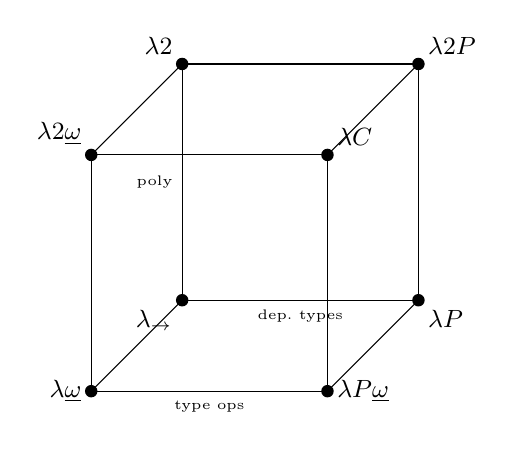
\begin{tikzpicture}[scale=1.5, every node/.style={font=\small}]
  \coordinate (lto) at (0,0,0);
  \coordinate (lP)  at (2,0,0);
  \coordinate (l2)  at (0,2,0);
  \coordinate (lw)  at (0,0,2);
  \coordinate (lPw) at (2,0,2);
  \coordinate (l2P) at (2,2,0);
  \coordinate (l2w) at (0,2,2);
  \coordinate (lC)  at (2,2,2);

  \fill (lto) circle (1.5pt); \node[below left]  at (lto) {$\lambda_\to$};
  \fill (lP)  circle (1.5pt); \node[below right] at (lP)  {$\lambda P$};
  \fill (l2)  circle (1.5pt); \node[above left]  at (l2)  {$\lambda 2$};
  \fill (lw)  circle (1.5pt); \node[left]         at (lw)  {$\lambda\underline\omega$};
  \fill (lPw) circle (1.5pt); \node[right]        at (lPw) {$\lambda P\underline\omega$};
  \fill (l2P) circle (1.5pt); \node[above right] at (l2P) {$\lambda 2P$};
  \fill (l2w) circle (1.5pt); \node[above left]  at (l2w) {$\lambda 2\underline\omega$};
  \fill (lC)  circle (1.5pt); \node[above right] at (lC)  {$\lambda C$};

  \draw[thin] (lto)--(lP) node[midway,below,font=\tiny]{dep.\ types};
  \draw[thin] (lto)--(l2) node[midway,left,font=\tiny]{poly};
  \draw[thin] (lto)--(lw);
  \draw[thin] (lP)--(l2P);
  \draw[thin] (lP)--(lPw);
  \draw[thin] (l2)--(l2P);
  \draw[thin] (l2)--(l2w);
  \draw[thin] (lw)--(lPw) node[midway,below,font=\tiny]{type ops};
  \draw[thin] (lw)--(l2w);
  \draw[thin] (lPw)--(lC);
  \draw[thin] (l2P)--(lC);
  \draw[thin] (l2w)--(lC);
\end{tikzpicture}
\caption{The $\lambda$-cube. Axes correspond to types depending on terms (depth),
terms depending on types (height), and types depending on types (width). The
Calculus of Constructions $\lambda C$ occupies the top vertex.}
\end{figure}

This interpretation of the cube as a coordinate system for dependency relations
carries the key insight: the cube does not classify programming languages. It
describes the minimal skeleton of cross-level dependency relations needed for a
formal system to be self-describing. Any system capable of expressing objects,
their constraints, and the constraints on those constraints must acquire
structures equivalent to the three axes of the cube. The neural network context
makes this resonance visible: neural networks are precisely systems whose
internal representations describe constraints over input manifolds, and the
$\lambda$-cube describes the minimal architecture for reasoning about such
constraint hierarchies.

%% ======================================================================
\section{Comprehension Categories and the Emergence of the Cube}
%% ======================================================================

The fact that the $\lambda$-cube arises naturally from minimal categorical
data is made precise by the theory of comprehension categories. A comprehension
category provides the minimal structural account of the relationship between
contexts, types, and terms, and from this account the cube's structure emerges
automatically.

\begin{definition}[Comprehension Category]
A \emph{comprehension category} consists of a fibration $p : \E \to \C$
together with, for every object $A$ lying over $\Gamma$ in $\E$, a chosen
morphism
\[
\chi_A \;:\; \Gamma.A \;\longrightarrow\; \Gamma
\]
in $\C$, called the \emph{context extension} map, with the property that the
pullback of $A$ along $\chi_A$ is the generic element of $A$.
\end{definition}

The base category $\C$ represents contexts: its objects are environments $\Gamma
= (x_1 : A_1, \dots, x_n : A_n)$, and its morphisms are substitutions between
contexts. The total category $\E$ contains dependent types together with their
context information. A type judgment $\Gamma \vdash A : *$ corresponds to an
object $A \in \E$ with $p(A) = \Gamma$. The context extension $\Gamma.A$ is
the context obtained by adding a fresh variable of type $A$; the comprehension
map $\chi_A$ expresses the projection forgetting that variable. Geometrically,
$\Gamma.A$ behaves like the total space of a bundle whose base is $\Gamma$ and
whose fiber at each point consists of the possible values of $A$.

This minimal structure generates the fundamental operations of type theory
through adjunctions. Given a substitution $f : \Delta \to \Gamma$, the
fibration provides a reindexing functor $f^* : \E_\Gamma \to \E_\Delta$.
Dependent products appear when this functor possesses a right adjoint:
\[
\Pi_f \;\dashv\; f^*.
\]
The right adjoint $\Pi_f$ maps a type $B$ over $\Delta$ to a type $\Pi_f B$
over $\Gamma$ that aggregates all coherent selections from $B$---the space
of sections of the bundle. Dependent sums appear as the corresponding left
adjoint:
\[
f^* \;\dashv\; \Sigma_f,
\]
constructing the total space by pairing each base element with an element of
its fiber. When both adjoints exist for every projection in the fibration,
the comprehension category models a locally cartesian closed category.

Once this structure is in place, the three axes of the $\lambda$-cube emerge
automatically from the question of how many levels of the comprehension
structure may serve as bases for further comprehension. Allowing types to serve
as bases for further type families introduces the dependent-type axis. Allowing
types to parameterize terms polymorphically introduces the polymorphism axis.
Allowing types to depend on other types introduces the type-operator axis. The
Calculus of Constructions arises when all three levels may serve as base spaces
for fibrations and the comprehension structure is closed under all three forms
of dependency.

The cube is therefore not a classification imposed from outside but a structure
that grows organically from the minimal categorical data of a comprehension
category. It is the dependency skeleton of any self-describing formal system.

%% ======================================================================
\section{Grothendieck Fibrations and the Geometry of Dependent Types}
%% ======================================================================

The connection between type theory and Grothendieck fibrations is where the
geometric interpretation of logic becomes fully explicit.

\begin{definition}[Grothendieck Fibration]
A functor $p : \E \to \B$ is a \emph{Grothendieck fibration} if for every
object $e \in \E$ and every morphism $f : b \to p(e)$ in $\B$, there exists a
\emph{cartesian lifting}: a morphism $\bar f : \bar b \to e$ in $\E$ with
$p(\bar f) = f$, through which every other morphism over $f$ factors uniquely.
\end{definition}

The base category $\B$ represents contexts. For each $\Gamma \in \B$, the
fiber category $\E_\Gamma$ is the category of types in context $\Gamma$. The
correspondence with type-theoretic judgments is nearly perfect:
\begin{align*}
\Gamma \in \B \quad &\longleftrightarrow \quad \text{a context} \\[2pt]
A \in \E_\Gamma \quad &\longleftrightarrow \quad \Gamma \vdash A : * \\[2pt]
t \in \E_\Gamma(A, B) \quad &\longleftrightarrow \quad \Gamma \vdash t : A \to B
\end{align*}
A morphism $f : \Delta \to \Gamma$ in the base induces a reindexing functor
$f^* : \E_\Gamma \to \E_\Delta$ via cartesian lifting. This is substitution.

The dependent product $\Pi_{x:A} B(x)$ arises as the right adjoint of
reindexing along the projection $p_A : \Gamma.A \to \Gamma$:
\[
\begin{tikzcd}
\E_{\Gamma.A} \arrow[r, shift left=2, "\Pi_{p_A}"] &
\E_\Gamma \arrow[l, shift left=2, "p_A^*"'] \arrow[l, phantom, "\dashv"]
\end{tikzcd}
\]
The right adjoint assembles all coherent sections of the bundle into a single
object. In logical terms this is universal quantification; in geometric terms it
is the space of sections of a fiber bundle. The dependent sum $\Sigma_{x:A}
B(x)$ appears as the left adjoint, constructing the total space.

Under sheaf semantics this structure acquires additional geometric content. A
context acts like an open region of a base space, a type describes how objects
vary across that region, and a term is a consistent section. Logical proof
becomes the construction of global sections from local constraints. The
subject-reduction property of typed calculi---the fact that evaluation preserves
typing---is the condition that the evaluation flow remains within the fibers of
the fibration, never leaving the constraint manifold defined by the type.

%% ======================================================================
\section{The $\lambda$-Cube as a Lattice of Adjunctions}
\label{sec:adjunctions}
%% ======================================================================

The deepest way to understand the $\lambda$-cube is through adjoint functors.
Each axis of the cube corresponds to a distinct adjoint pair becoming available
inside the internal language.

The simply typed $\lambda$-calculus $\lambda_\to$ lives in a cartesian closed
category. The function type $A \to B$ is the exponential $B^A$, and the currying
isomorphism
\[
\Hom(X \times A,\, B) \;\cong\; \Hom(X,\, B^A)
\]
expresses the adjunction $(- \times A) \dashv (-)^A$. The $\lambda$-abstraction
rule is the internal language of this adjunction.

The dependent-type axis introduces, for each projection $p_A : \Gamma.A \to
\Gamma$, the triple adjunction
\[
\Sigma_{p_A} \;\dashv\; p_A^* \;\dashv\; \Pi_{p_A}.
\]
This corresponds to the categorical transition from cartesian closed categories
to locally cartesian closed categories. The polymorphism axis introduces the
ability to quantify over the universe of types, requiring the universe to be
treated as an object and polymorphic terms to correspond to natural
transformations. The type-operator axis introduces internal hom-objects at the
level of types, adding exponentials between kinds.

The Calculus of Constructions $\lambda C$ occupies the vertex where all three
adjoint structures coexist. The Curry--Howard--Lambek correspondence makes the
full triangulation explicit:

\begin{center}
\begin{tabular}{lll}
\toprule
\textbf{Logic} & \textbf{Type Theory} & \textbf{Category Theory} \\
\midrule
Propositions & Types & Objects \\
Proofs & Terms & Morphisms \\
Universal quantification & $\Pi$-type & Right adjoint to reindexing \\
Existential quantification & $\Sigma$-type & Left adjoint to reindexing \\
Implication & Function type & Exponential / internal hom \\
Substitution & $\beta$-reduction & Adjoint transpose \\
\bottomrule
\end{tabular}
\end{center}

The adjoint lattice extends naturally beyond three dimensions. Modal type
theories arise from adjunctions between modalities and inclusion functors.
Linear type theories arise from adjunctions between tensor products and linear
internal homs. Universe hierarchies $\Type_0 : \Type_1 : \Type_2 : \cdots$
arise from adjunctions between universe levels. The $\lambda$-cube is the
three-dimensional shadow of this larger structure: the most visible
cross-section because it is the minimal one containing all three fundamental
modes of dependency.

%% ======================================================================
\section{Type Theory as Information Geometry}
\label{sec:infogeo}
%% ======================================================================

Once the $\lambda$-cube is interpreted geometrically as a space of constraints
and flows, its structure becomes comparable to the manifolds studied in
information geometry and statistical field theory. The comparison reveals that
typed computation and statistical inference share a common geometric skeleton.

In information geometry, a statistical model is a Riemannian manifold whose
coordinates parameterize probability distributions. A point corresponds to a
particular distribution; a curve corresponds to a continuous transformation of
that distribution. The Fisher information metric equips the manifold with an
intrinsic notion of distance, and divergence measures define the geodesic
structure. Learning and inference are motion through this manifold.

The typing judgment $\Gamma \vdash t : T$ can be interpreted in a parallel way.
The context $\Gamma$ specifies a coordinate system; $T$ defines a constraint
surface within the space of program states; and the judgment asserts that $t$
lies on that surface. Beta reduction in the $\lambda$-calculus is a dynamical
flow on this space: each reduction step transforms a term while preserving its
type, so the flow remains on the constraint manifold. The subject-reduction
theorem is the condition that the flow never leaves the manifold.

Dependent types introduce fiber bundle structure. A family $x : A \vdash B(x)$
defines a bundle over $A$ whose fiber at each $a$ is the constraint manifold
$B(a)$. A dependent function of type $\Pi_{x:A} B(x)$ is a section. This is
the exact structure of a physical field: a field assigns to each spacetime event
an element of a fiber determined by the gauge structure. The $\Pi$-type performs
the same role as integration of a field over a base space.

The $\lambda$-cube describes which kinds of fields over constraint manifolds are
permitted. The dependent-type axis allows the constraint manifold to vary with
the base point. The polymorphism axis allows programs to be uniform across the
entire universe of manifolds. The type-operator axis allows manifolds to depend
on other manifolds. The Calculus of Constructions permits fields over fields
over fields, allowing constraints, programs, and meta-structures to interact
recursively. In information-geometric terms, the system can describe statistical
models over statistical models---manifolds parameterized by manifolds.

%% ======================================================================
\section{Homotopy Type Theory and the Extension Beyond the Cube}
\label{sec:hott}
%% ======================================================================

Homotopy type theory (HoTT) demonstrates that the geometric interpretation of
type theory can be pushed to the point where the logic of type theory and the
logic of homotopy theory become provably equivalent. In HoTT, types are
topological spaces, elements are points, and equality proofs are paths. The
identity type $\mathrm{Id}_A(a, b)$ is the space of paths from $a$ to $b$ in
$A$. Higher identity types correspond to surfaces connecting paths, and so on.

Under this interpretation, dependent types become genuine fibrations in the
topological sense. The family $x : A \vdash B(x)$ is a continuous map from the
total space $\Sigma_{x:A} B(x)$ to the base $A$ with the standard path-lifting
properties. The $\Pi$-type is the space of sections of this fibration.

The univalence axiom asserts that equivalent types are identical. In categorical
terms, the identity type of the universe is homotopy equivalent to the space of
type equivalences. The universe therefore carries the structure of a classifying
space: paths are equivalences, surfaces are natural isomorphisms, and
higher-dimensional cells are higher coherences.

Higher topos theory provides the categorical framework for this extension. An
$(\infty, 1)$-topos is a category whose internal language is precisely HoTT.
The $\lambda$-cube describes the internal language of an ordinary topos---the
$0$-dimensional case---while HoTT describes the internal language of an
$(\infty, 1)$-topos. Between these extremes lie the internal languages of
$n$-toposes for each natural number $n$, forming an infinite hierarchy extending
the cube in a direction orthogonal to all three of its original axes.

Derived algebraic geometry extends this picture further. The $\lambda$-cube
therefore appears, in the longest view, as the minimal coordinate patch of an
infinite-dimensional space of type theories parameterized by their homotopical
dimension and homological depth.

%% ======================================================================
\section{Representation Learning as a Renormalization Flow}
\label{sec:renorm}
%% ======================================================================

The geometric interpretation of neural representation spaces admits a natural
analogy with renormalization group (RG) flows in statistical physics. In both
settings a complex high-dimensional system is described at multiple levels of
resolution, and the effective behavior observed at a given scale depends on how
fine-grained degrees of freedom have been integrated out.

Let $h_\theta : X \to \mathbb{R}^d$ denote the representation map parameterized
by $\theta$. Training modifies $\theta$ through gradient descent, producing a
trajectory
\[
\theta_0 \;\longrightarrow\; \theta_1 \;\longrightarrow\; \cdots
\]
that induces a corresponding evolution of representation geometries. At early
stages of training the representation map tends to preserve fine-grained
variations in the input. As training progresses, the model learns to collapse
directions irrelevant to the task---the small-singular-value directions discussed
in the spectral analysis above. This collapse is directly analogous to the
separation of relevant and irrelevant operators under renormalization group flow.
Relevant operators dominate the large-scale behavior; irrelevant operators decay
under coarse-graining.

The foliation structure of representation space emerges as a fixed point of this
renormalization-like process. Directions associated with small singular values
form the tangent bundle of the semantic equivalence foliation. Directions
associated with large singular values define the transverse bundle along which
classification changes occur. Training flows the system toward a configuration
in which this spectral separation is maximized, just as RG flows drive a system
toward a fixed point by integrating out high-frequency fluctuations.

This perspective also clarifies the scaling behavior of adversarial
transferability. As model size increases, the dimensionality of the
representation manifold grows and the number of relevant directions increases.
However, independently trained models tend to develop different orientations for
their relevant subspaces. In high-dimensional spaces the expected overlap
between two adversarial subspaces $U_S$ and $U_T$ scales as $1/d$, so larger
models possess richer adversarial geometry but lower cross-model alignment. The
renormalization interpretation suggests that large models develop
non-renormalizable degrees of freedom---gradient directions that cannot be
described by a simple shared effective theory---which is why their adversarial
directions decorrelate across independently trained instances.

Within the broader framework developed in this essay, this renormalized
representation manifold functions as a constraint field over the space of inputs.
Neural inference corresponds to evaluating sections of this field; adversarial
perturbations correspond to trajectories that leave the local constraint leaf
and move along unstable transverse directions. Seen from this perspective,
representation learning, dependent type theory, and categorical semantics all
describe systems in which structures evolve under constraint-preserving flows.
The renormalization analogy provides a physical intuition for the essay's central
claim: intelligence, logic, and learning are all governed by the geometry of
constraint fields defined over spaces of contexts.

%% ======================================================================
\section{Semantic Manifolds and the Emergence of Adversarial Cones}
\label{sec:cones}
%% ======================================================================

The geometric framework developed throughout this essay allows gradient-based
adversarial attacks to be interpreted as natural differential-geometric
operations on the representation manifold: they are first-order approximations
to geodesic escape from the leaves of the semantic foliation.

Let $F = f \circ h : X \to \mathbb{R}^k$ be the composed classifier and let
$\mathcal{F}$ be the foliation induced by training. At each point $x$, the
tangent space $T_x \mathcal{F}$ consists of directions that leave the
classification invariant to first order, while the transverse bundle $A_x =
(T_x \mathcal{F})^\perp$ contains the adversarially sensitive directions
(Theorem~\ref{thm:adversarial}).

A gradient-based adversarial attack computes the direction of steepest ascent
of the loss under a norm constraint. The sign perturbation
\[
\delta^* \;=\; \epsilon\,\sign(\nabla_x L(x))
\]
approximates the projection of $\nabla_x L(x)$ onto the $\ell_\infty$ unit
sphere. Since $\nabla_x L(x) \in A_x$ (it is orthogonal to the leaf tangent
space), this perturbation moves the input in the adversarially sensitive
direction: the transverse escape direction of the foliation.

The set of all such directions at $x$ forms the \emph{adversarial cone}:
\[
C_x \;=\; \bigl\{ v \in T_x X \;\mid\;
\langle \nabla_x L(x),\, v \rangle > 0 \bigr\}.
\]
In high-dimensional spaces this half-space occupies a large fraction of the
ambient tangent space. Consequently, randomly sampled perturbations have
non-negligible probability of falling within $C_x$, which explains the
empirical abundance of adversarial examples.

The geometry becomes particularly striking near singular strata, where $\dim
T_x \mathcal{F}$ decreases discontinuously. At such points the transverse
bundle expands abruptly and the adversarial cone widens. These are precisely the
unstable classification boundaries at which adversarial examples cluster most
densely. Robustness is therefore equivalent to increasing the geodesic distance
from typical data points to the nearest singular stratum of the foliation: a
network is adversarially robust insofar as a significant geodesic displacement
is required to escape the local leaf.

The connection to adversarial transfer is now geometric and explicit. Two models
$S$ and $T$ have similar adversarial cones when their foliation tangent bundles
are aligned. CKA measures this alignment. A high-CKA surrogate shares the
foliation geometry of the target, so attacks computed by following $\nabla_x
L_S(x)$ lie in the adversarial cone of $T$ as well. A low-CKA surrogate has
rotated adversarial cones, and transfer fails because $\nabla_x L_S(x)$ is
orthogonal to the sensitive directions of $T$. The Cox--Bunzel protocol, by
combining both families of surrogates, covers adversarial cones from multiple
orientations and thereby provides representative coverage of the full transverse
bundle of the target.

%% ======================================================================
\section{Geometric Summary Theorem}
\label{sec:summary}
%% ======================================================================

The analysis developed throughout this essay can be unified into a single formal
statement that makes the central claim of the paper precise.

\begin{theorem}[Geometry of Constraints]
\label{thm:main}
Let $\mathfrak{S}$ denote any of the following three classes of system:
\begin{enumerate}[label=\emph{(\roman*)}]
\item A trained neural network with representation map $h : X \to \mathbb{R}^d$;
\item A dependent type theory presented as a comprehension category
      $p : \E \to \C$ with context extension;
\item A family of statistical models presented as a fibered manifold over a
      base of parameters.
\end{enumerate}
In each case there exists a structure of the following kind:
\begin{enumerate}[label=\emph{(\alph*)}]
\item A \emph{base space of contexts} $B$, whose points parameterize the
      local conditions under which the system operates.

\item A \emph{constraint field} over $B$: a Grothendieck fibration
      $p : \E \to B$ whose fiber $\E_b$ over context $b$ is the space of
      admissible states or types under condition $b$.

\item A \emph{canonical section} $s : B \to \E$ describing the globally
      coherent behavior of the system, satisfying $p \circ s = \mathrm{id}_B$.

\item A \emph{foliation} $\mathcal{F}$ of the total space $\E$ into leaves
      of approximate equivalence, induced by the task structure or type
      constraints. The tangent bundle $T\mathcal{F}$ encodes the directions
      along which the system's output is invariant; the transverse bundle
      $T\E / T\mathcal{F}$ encodes the directions of sensitivity.

\item An \emph{instability locus}: the singular strata of $\mathcal{F}$,
      where the leaf dimension drops and the transverse bundle expands.
      In neural networks these are the adversarial boundaries; in type theory
      these are the boundaries between normal and stuck computation; in
      information geometry these are the boundaries of statistical
      distinguishability.
\end{enumerate}

The system is \emph{robust} insofar as the section $s$ avoids the
instability locus: the geodesic distance from $s(b)$ to the nearest
singular stratum, measured in the pullback metric induced by the
Jacobian of the section, is large. The characteristic failure modes of
each domain---adversarial perturbations, type errors, and statistical
non-identifiability---correspond to different mechanisms by which the
section approaches or crosses a singular stratum.

Moreover, when two systems of the same class are compared, their
\emph{structural similarity} (measured by CKA in neural networks,
by natural isomorphism of fiber categories in type theory, or by
statistical distance of the corresponding fibered manifolds) predicts
the degree to which the transverse bundles of their respective sections
are aligned, and hence the degree to which instabilities in one system
transfer to the other.
\end{theorem}

\begin{proof}[Proof sketch]
Parts (a)--(c) hold for neural networks by the fiber bundle construction
of Section~\ref{sec:bundles} and the Grothendieck fibration formalization
in the appendix. Parts (a)--(c) hold for comprehension categories by
definition and for statistical manifolds by the Grothendieck construction
applied to the functor assigning fiber manifolds to base parameters.

Part (d) holds for neural networks by the spectral analysis of the Jacobian
(the foliation is induced by the kernel of $D(f \circ h)$) and for
comprehension categories by the fibered structure of the type theory (the
foliation is induced by definitional equality in the fibers). Part (e) is
Theorem~\ref{thm:adversarial} in the neural setting and corresponds to
non-normal-form terms in the type-theoretic setting.

Robustness follows from the geodesic interpretation of adversarial attacks
in Section~\ref{sec:cones}: a perturbation produces a singular crossing if
and only if the geodesic distance in the pullback metric from the current
section value to the instability locus is less than the perturbation radius.
Structural similarity and transferability are related by the foliation
alignment argument of Section~\ref{sec:foliation}: aligned foliations have
aligned transverse bundles, and perturbations effective in one system lie in
the adversarial cone of the other. \qed
\end{proof}

\begin{remark}
Theorem~\ref{thm:main} should be understood as a structural theorem rather
than a quantitative one: it identifies the common architecture underlying
three domains without specifying uniform quantitative bounds across them. The
quantitative theory specific to each domain (NP-hardness results for adversarial
verification, coherence conditions for comprehension categories, and Fisher
information bounds for statistical distinguishability) is richer than what a
single unified theorem can encode. The theorem's value lies in identifying the
shared geometric vocabulary that makes each domain's quantitative results
interpretable in the others.
\end{remark}

%% ======================================================================
\section{Returning to Machine Learning: Constraint Fields in Practice}
%% ======================================================================

With the full theoretical framework in place it is possible to revisit the
applied problem of adversarial robustness and state precisely what the
geometric theory contributes to its solution.

A trained neural network defines a representation field over its input space.
At each input $x$, the network's internal state $h_M(x) \in \mathbb{R}^d$
is the value that the representation field assigns to $x$. The training process
shapes this field to assign similar values to semantically similar inputs,
encoding the task geometry in the structure of the field.

Under the fibration interpretation established in Theorem~\ref{thm:main}, the
network's representation is a section of a bundle over input space whose
fiber-smoothness properties determine the model's adversarial behavior.
CKA-based representational similarity is a probe of fibrational alignment
between two networks: high CKA indicates that the respective sections organize
the input manifold into similar geometric patterns, so the adversarial cones
are aligned and attacks transfer. The Cox--Bunzel testing protocol is a strategy
for obtaining representative coverage of the adversarial cone by sampling
surrogates from both aligned and orthogonal orientations.

The renormalization interpretation of Section~\ref{sec:renorm} suggests that
the most robust possible network is one whose representation field has been
trained to its fixed-point configuration: one in which the semantic foliation
is maximally sharp (large spectral gap in the Jacobian singular values) and
maximally stable (the instability locus is far from typical data points in
the pullback metric). This corresponds to a model whose constraint field is
strongly laminar---varying rapidly in a small number of task-relevant directions
and negligibly in all others---so that adversarial perturbations require a large
geodesic step to reach the instability locus.

The challenge of AI robustness is, at its deepest level, the challenge of
understanding and controlling the geometry of representation spaces as constraint
fields over the manifold of possible inputs. The techniques developed for this
problem---CKA-based representational similarity, surrogate partitioning, diagonal
box metrics---are instruments for probing the geometry of learned constraint
fields. The geometric framework of this essay provides the conceptual vocabulary
in which those instruments can be combined into a coherent theory.

%% ======================================================================
\section{Convergence: The Geometry of Constraints}
\label{sec:convergence}
%% ======================================================================

This essay has traced a path from adversarial examples through representation
geometry, foliation theory, Jacobian spectral analysis, transformer attention
as a dynamic metric, categorical semantics, Grothendieck fibrations,
comprehension categories, the $\lambda$-cube and its adjoint lattice,
information geometry, homotopy type theory, renormalization flows, and the
derivation of adversarial cones as geodesic escape directions. The diversity
of these topics conceals a structural unity that the foregoing analysis has
progressively revealed and Theorem~\ref{thm:main} has formalized.

The unity can be stated as a single organizing claim: complex systems---whether
machine learning models, typed programming languages, or mathematical proof
systems---are best understood as layered spaces of states, constraints, and
meta-constraints, and the phenomena characteristic of each domain are instances
of motion through such layered spaces under the governance of their constraint
geometry.

In machine learning, states are input representations; constraints are the
typing-like conditions imposed by training objectives and architectural inductive
biases; adversarial vulnerability is the existence of transverse directions along
which small motion produces large change in behavioral category; and robustness
evaluation is the problem of characterizing the geometry of these transverse
directions without complete knowledge of the full constraint field.

In type theory, states are program terms; constraints are types (constraint
manifolds in the state space); computation is motion along those manifolds
governed by reduction rules; and the $\lambda$-cube describes the minimal
configuration of cross-level dependencies needed for a language to reason about
itself.

In categorical semantics, the same structure appears as a Grothendieck
fibration: a functor from a total category of constrained objects to a base
category of contexts, equipped with reindexing functors and their adjoints. The
fibration encodes, in categorical language, exactly the structure of
substitution, dependent quantification, and context extension that type theory
requires syntactically.

In information geometry, the structure appears as a family of statistical
manifolds parameterized by a base space of models, with sections corresponding
to consistent statistical inferences across the family.

What appears initially as a collection of unrelated technical tools---adversarial
testing frameworks, dependent type systems, categorical fibrations, information
geometry---is, under the analysis developed here, a collection of partial
descriptions of the same underlying mathematical object: a geometry of
constraints governing how structures vary across contexts and interact across
levels of abstraction. The $\lambda$-cube, Grothendieck fibrations, and neural
representation manifolds are, each in their own register, charts for different
regions of this geometry. The enterprise of understanding any one of them in
depth is, in the end, the same enterprise as understanding all the others.

%% ======================================================================
\appendix
\section{Neural Representation Maps as Sections of a Grothendieck Fibration}
%% ======================================================================

This appendix makes explicit the categorical construction promised in
Section~\ref{sec:bundles}. The goal is to demonstrate, without appeal to
metaphor, that a neural representation map is a section of a Grothendieck
fibration over input contexts in the same formal sense that a dependent-type
term is a section of the comprehension fibration.

\subsection*{Construction of the Base Category}

Let $X$ denote the input space of a neural network. Define a category $\B$
whose objects are \emph{input contexts}: pairs $(U, \mathcal{T})$ where $U
\subseteq X$ is a measurable region and $\mathcal{T}$ is a set of admissible
transformations of $U$ (preprocessing operations, token substitutions,
perturbations of bounded norm). A morphism
\[
f : (U, \mathcal{T}) \;\longrightarrow\; (V, \mathcal{T}')
\]
is an admissible map $f : U \to V$ that intertwines the transformation
structures: $\mathcal{T}' \circ f \subseteq f \circ \mathcal{T}$. Composition
is ordinary function composition; identity morphisms are inclusions. The
category $\B$ captures the space of contexts over which the network operates.

\subsection*{Construction of the Total Category and Projection}

Define the total category $\E$ whose objects are triples $(U, \mathcal{T}, r)$
with $(U, \mathcal{T}) \in \B$ and $r : U \to \mathbb{R}^d$ a measurable
representation assignment over that context. A morphism
\[
(U, \mathcal{T}, r) \;\longrightarrow\; (V, \mathcal{T}', r')
\]
consists of a base morphism $f : (U, \mathcal{T}) \to (V, \mathcal{T}')$
together with a commutation condition: $r = r' \circ f$ (the representation
over $U$ is the pullback of the representation over $V$ along $f$). The
projection functor $p : \E \to \B$ is defined by
\[
p(U, \mathcal{T}, r) \;=\; (U, \mathcal{T}), \qquad
p(f, \mathrm{comm.}) \;=\; f.
\]

\subsection*{Verification of the Fibration Property}

For each object $(U, \mathcal{T}, r')$ of $\E$ and each morphism $f :
(U, \mathcal{T}) \to (V, \mathcal{T}')$ in $\B$, define the pullback
representation
\[
f^* r' \;=\; r' \circ f \;:\; U \;\longrightarrow\; \mathbb{R}^d.
\]
The morphism $(U, \mathcal{T}, f^* r') \to (V, \mathcal{T}', r')$ consisting
of $(f, \mathrm{id}_{r' \circ f})$ is cartesian: every morphism $(W, \mathcal{T}'',
r'') \to (V, \mathcal{T}', r')$ in $\E$ lying over a morphism $g : (W,
\mathcal{T}'') \to (U, \mathcal{T})$ in $\B$ factors uniquely through the
pullback. This is precisely the universal property of cartesian liftings.
The functor $p$ is therefore a Grothendieck fibration.

\subsection*{The Neural Network as a Section}

The neural network with representation map $h : X \to \mathbb{R}^d$ determines
a section $s : \B \to \E$ of this fibration:
\[
s(U, \mathcal{T}) \;=\; (U, \mathcal{T},\, h|_U), \qquad
s(f) \;=\; (f, h|_U = h|_V \circ f).
\]
By construction $p \circ s = \mathrm{id}_\B$, confirming that $s$ is a section.
The commutativity condition $h|_U = h|_V \circ f$ holds automatically for any
admissible $f$, because $h$ is defined globally on $X$ and $h|_U$ is simply
its restriction. The section is therefore well-defined.

\subsection*{Adversarial Perturbations as Base Morphisms}

An adversarial perturbation of bounded norm $\epsilon$ at input $x \in U$
defines a morphism in $\B$:
\[
\delta : (U, \mathcal{T}) \;\longrightarrow\; (U_\epsilon, \mathcal{T}_\epsilon)
\]
where $U_\epsilon$ is the $\epsilon$-ball around $x$ and $\delta$ maps $x$ to
$x + v$ for some $v$ with $\|v\| \leq \epsilon$. The total displacement induced
by $s$ along this morphism is
\[
s(U_\epsilon, \mathcal{T}_\epsilon) \;=\;
(U_\epsilon, \mathcal{T}_\epsilon,\, h|_{U_\epsilon}).
\]
The adversarial perturbation is effective when $h(x + v) - h(x)$ is large
relative to $\|v\|$, which is equivalent to saying that the section $s$ has
a large derivative in the direction $v$: the morphism $\delta$ induces a large
displacement in the fiber $\mathbb{R}^d$ through the section. This is
precisely the condition---section gradient large in the transverse direction---
identified in Theorem~\ref{thm:adversarial}.

\subsection*{Interpretation}

This construction demonstrates that the neural network's representation map
occupies the same formal role as a term inhabiting a dependent type: both are
sections of Grothendieck fibrations assigning values consistently across a space
of contexts. The base category of input contexts corresponds to the base category
of typing contexts; the fiber of representation assignments corresponds to the
fiber of type-admissible terms; the pullback reindexing corresponds to
substitution; and adversarial perturbations correspond to context morphisms that
produce large fiber displacements through the section. The geometric problem
of adversarial robustness---controlling how sections behave under base
category morphisms---is formally identical to the problem of ensuring that
term-evaluation is stable under context change, which is the subject-reduction
problem of type theory.

%% ======================================================================
\begin{thebibliography}{99}

\bibitem{goodfellow2015} Goodfellow, I., Shlens, J., and Szegedy, C. (2015).
Explaining and harnessing adversarial examples. \textit{International Conference
on Learning Representations}.

\bibitem{szegedy2014} Szegedy, C., et al. (2014). Intriguing properties of
neural networks. \textit{International Conference on Learning Representations}.

\bibitem{kornblith2019} Kornblith, S., Norouzi, M., Lee, H., and Hinton, G.
(2019). Similarity of neural network representations revisited. \textit{ICML},
3519--3529.

\bibitem{papernot2016} Papernot, N., McDaniel, P., and Goodfellow, I. (2016).
Transferability in machine learning: From phenomena to black-box attacks using
adversarial samples. \textit{arXiv:1605.07277}.

\bibitem{coxbunzel} Cox, B. and Bunzel, A. (2024). Adversarial robustness
evaluation and representational similarity. Manuscript.

\bibitem{euaiact} European Parliament and Council (2024). \textit{Regulation
on Artificial Intelligence (AI Act)}. Official Journal of the European Union.

\bibitem{barendregt1992} Barendregt, H. (1992). Lambda calculi with types.
In \textit{Handbook of Logic in Computer Science}, Vol.~2. Oxford University
Press.

\bibitem{jacobs1999} Jacobs, B. (1999). \textit{Categorical Logic and Type
Theory}. Elsevier.

\bibitem{grothendieck1960} Grothendieck, A. (1960). \'El\'ements de g\'eom\'etrie
alg\'ebrique. \textit{Publications Math\'ematiques de l'IH\'ES}, 4:5--214.

\bibitem{streicher1991} Streicher, T. (1991). \textit{Semantics of Type Theory}.
Birkh\"auser.

\bibitem{hofmann1994} Hofmann, M. (1994). On the interpretation of type theory
in locally cartesian closed categories. \textit{Computer Science Logic},
Lecture Notes in Computer Science.

\bibitem{univalent2013} Univalent Foundations Program (2013). \textit{Homotopy
Type Theory: Univalent Foundations of Mathematics}. Institute for Advanced Study.

\bibitem{lurie2009} Lurie, J. (2009). \textit{Higher Topos Theory}. Princeton
University Press.

\bibitem{amari2016} Amari, S. (2016). \textit{Information Geometry and Its
Applications}. Springer.

\bibitem{atiyah1989} Atiyah, M. (1989). Topological quantum field theory.
\textit{Publications Math\'ematiques de l'IH\'ES}, 68:175--186.

\bibitem{lawvere1969} Lawvere, F.W. (1969). Adjointness in foundations.
\textit{Dialectica}, 23(3--4):281--296.

\bibitem{seely1984} Seely, R. (1984). Locally cartesian closed categories and
type theory. \textit{Mathematical Proceedings of the Cambridge Philosophical
Society}, 95:33--48.

\bibitem{coquand1988} Coquand, T. and Huet, G. (1988). The Calculus of
Constructions. \textit{Information and Computation}, 76(2--3):95--120.

\bibitem{voevodsky2010} Voevodsky, V. (2010). Univalent foundations project.
Unpublished manuscript.

\bibitem{triantafillou2021} Triantafillou, E., et al. (2021). Representation
similarity in neural networks: A review. \textit{NeurIPS}.

\bibitem{madry2018} Madry, A., et al. (2018). Towards deep learning models
resistant to adversarial attacks. \textit{ICLR}.

\bibitem{carlini2017} Carlini, N. and Wagner, D. (2017). Towards evaluating
the robustness of neural networks. \textit{IEEE Symposium on Security and
Privacy}.

\bibitem{wilson1974} Wilson, K.G. and Kogut, J. (1974). The renormalization
group and the $\epsilon$ expansion. \textit{Physics Reports}, 12(2):75--199.

\bibitem{watanabe2009} Watanabe, S. (2009). \textit{Algebraic Geometry and
Statistical Learning Theory}. Cambridge University Press.

\bibitem{dieuleveut2022} Dieuleveut, A., et al. (2022). Bridging the gap
between singular learning theory and deep learning. \textit{arXiv:2208.00993}.

\bibitem{vafa2022} Vafa, K., et al. (2022). Unifying language learning
paradigms. \textit{arXiv:2205.05131}.

\end{thebibliography}

\end{document}
